
\subsection{Felix (Flexible blokken)}\label{felix}
Het is voor eindredacteuren mogelijk om blokken de plaatsen op pagina's. Hiermee krijgt de redacteur enige vrijheid over de indeling van de pagina. Hier zijn wel beperkingen van toepassing volgens het grafisch ontwerp.

Door met de muis over de grijze balk te gaan verschijnt er een tandwieltje, als je daarop klikt dan verschijnt er een optie \emph{Blok toevoegen}. Hier kan een keuze gemaakt worden om een enkel item weer te geven op de website, dit zijn \emph{Nodetypes}, of een aantal items, zoals bijvoorbeeld \emph{Het laatste nieuws}.

\begin{center}
	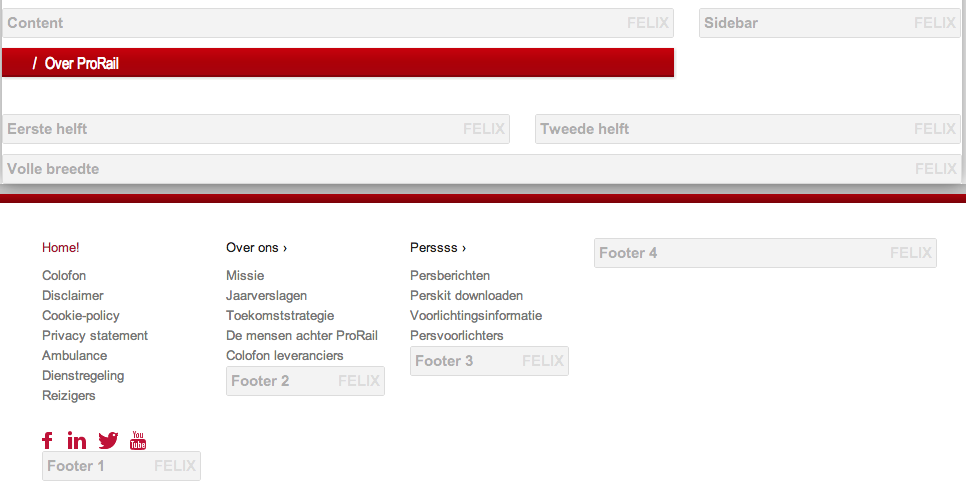
\includegraphics[width=\textwidth]{img/felix.png}
\end{center}

\subsubsection{Felix blok titel aanpassen}\label{felixbloktitel}

De titel van een felix blok kan altijd aangepast worden. Om dit te doen klik je op het \emph{tandwieltje} en vervolgens op \emph{Eigenschappen aanpassen}. Vul bij het veld \emph{Onderwerp} de gewenste titel in, laat het veld leeg om de standaard waarde te gebruiken. Klik op de knop \emph{Opslaan} om de titel op te slaan. 

\begin{center}
	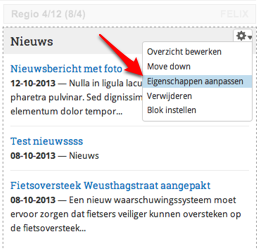
\includegraphics[scale=1.0]{img/felix0.png}
\end{center}

\subsubsection{Felix blok volgorde aanpassen}\label{felixblokvolgorde}

Klik op het \emph{tandwieltje} en klik vervolgens op \emph{Verplaats omhoog} of op \emph{Verplaats omlaag} om het blok 1 positie omhoog of omlaag te verplaatsen. De nieuwe blok volgorde zal automatisch opgeslagen worden.

\begin{center}
	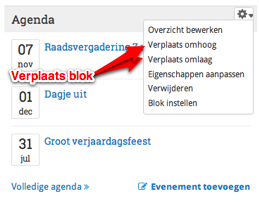
\includegraphics[scale=1.0]{img/felix3.png}
\end{center}

\subsubsection{Felix regio's}\label{felixregios}

De onderstaande afbeeldingen tonen alle felix regio's. Dit zijn gebieden op de website waar blokken aan toegevoegd kunnen worden. Op de afbeeldingen zie je aanduidingen als \emph{Regio 8/12} en \emph{Regio 4/12}, dit slaat op de breedte van de regio. De gehele pagina bestaat uit 12 kolommen, \emph{Regio 8/12} neemt dus 8 van de 12 kolommen in. Het is niet aangeraden om hele brede blokken (bijv. Carrousel breed 9/12) toe te voegen aan hele smalle regio's (bijv. Regio 4/12). Als je dit toch doet kan het zijn dat de opmaak van de website niet meer klopt.

\begin{center}
	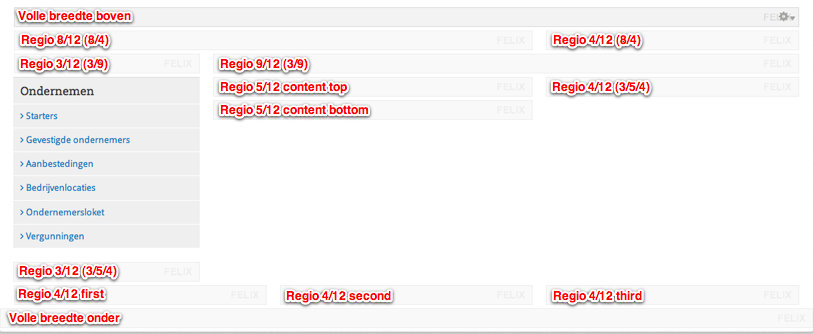
\includegraphics[width=\textwidth]{img/felix1.png}
\end{center}

\begin{center}
	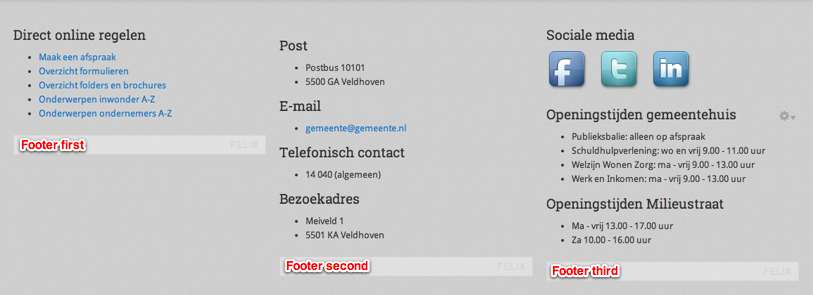
\includegraphics[width=\textwidth]{img/felix2.png}
\end{center}

\subsubsection{Felix blokken}\label{felixblokken}

Felix blokken zijn de daadwerkelijke flexibele blokken, deze specifieke blokken kunnen overal op de website en in alle felix regio's getoond worden.

\textbf{Nodetype}

\begin{itemize}
\item Editorial
\item Peiling
\item Slide 
\item Webformulier
\end{itemize}

\textbf{Block}

\begin{itemize}
\item Subnavigatie voorbeeld
\end{itemize}

\textbf{Menu}

\begin{itemize}
\item Toptaken
\end{itemize}

\textbf{Menu Block}

\begin{itemize}
\item Subnavigatie
\end{itemize}

\textbf{Quicktabs}

\begin{itemize}
\item Nieuws Agenda tabblok
\end{itemize}

\textbf{Submenu Tree}

\begin{itemize}
\item Sibling content
\item Extended menu links
\end{itemize}

\textbf{Views}

\paragraph{Agenda teaserblok}

Toont een lijst met 10 agendaitems. De volgende onderdelen zijn zichtbaar per agendaitem: titel (klikbaar), thumbnail (klikbaar), begindatum evenement en introtekst. Onderaan het blok zit paginering. Dit blok past optimaal in de middenkolom. Andere regio's zijn ook mogelijk het blok is responsive.

\begin{center}
	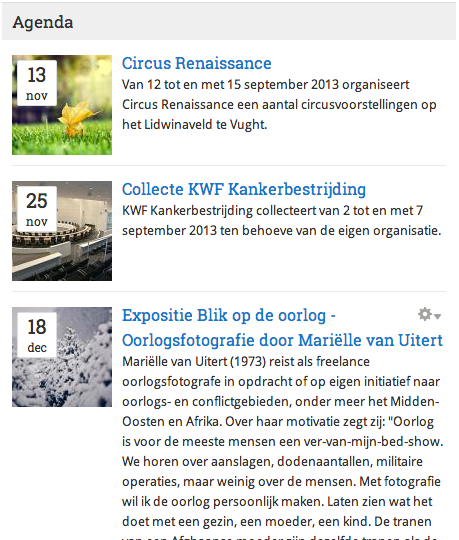
\includegraphics[scale=0.5]{img/blokken/agendateaser.png}
\end{center}

\paragraph{Agenda lijstblok}

Toont een lijst van 5 agendaitems. De volgende onderdelen zijn zichtbaar per agendaitem: titel (klikbaar) en begindatum evenement. Onderaan het blok zit staat een link naar de overzichtspagina en een link om agendaitems toe te voegen wanneer de juiste rechten beschikbaar zijn. Dit blok past optimaal in de rechterkolom. Andere regio's zijn ook mogelijk het blok is responsive.

\begin{center}
	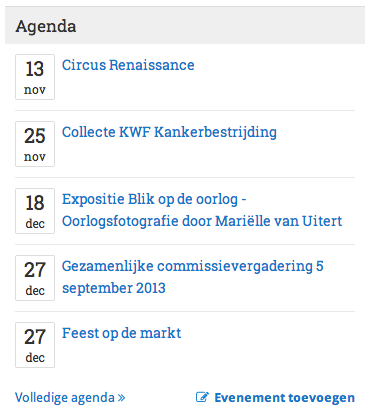
\includegraphics[scale=0.5]{img/blokken/agendalist.png}
\end{center}

\paragraph{Berichtenblok}

Toont een lijst van 5 berichten. De lijst bestaat uit klikbare titels die naar de detailpagina van het bericht gaan. Onderaan het blok staat een link naar de overzichtspagina.

\begin{center}
	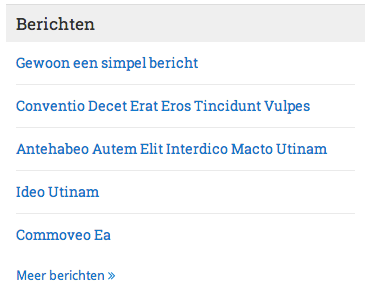
\includegraphics[scale=0.5]{img/blokken/berichten.png}
\end{center}

\paragraph{Teamdocumentenblok}

Toont een lijst van 5 bestanden. De volgende onderdelen zijn zichtbaar: extensie, naam van het document (klikbaar), bestandsgrootte, geupload door, geupload op.

\begin{center}
	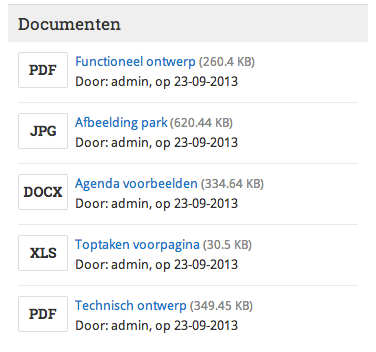
\includegraphics[scale=0.5]{img/blokken/teamdocumenten.png}
\end{center}

\paragraph{Favorietenblok}

Toont een lijst met 5 favorieten. Deze lijst bestaat uit klikbare titels die linken naar de detailpagina van het item.

\begin{center}
	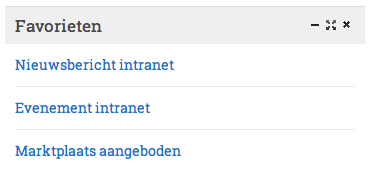
\includegraphics[scale=0.5]{img/blokken/favorieten.png}
\end{center}

\paragraph{Fotoalbumblok}\label{fotoalbumblok}

Het fotoalbumblok bestaat uit een lijst met gevulde fotoalbums. Door te klikken op een fotoalbum gaat men naar de albumoverzichtpagina met de beschikbare foto's.

\begin{center}
	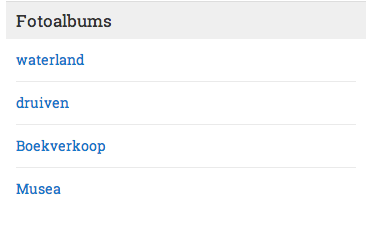
\includegraphics[scale=0.5]{img/blokken/fotoalbum.png}
\end{center}

\paragraph{Google maps kaart}

Toont een Google Maps kaart die de locatie toont op de kaart die opgegeven is bij een item. Dit blok wordt standaard getoont in de rechterkolom bij items die een locatie gekoppeld hebben.

\begin{center}
	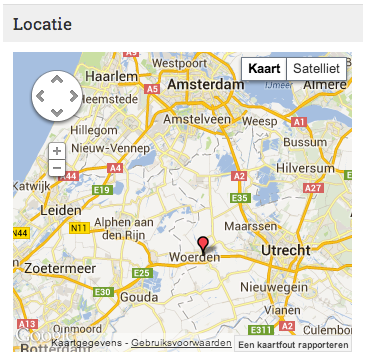
\includegraphics[scale=0.5]{img/blokken/googlemaps.png}
\end{center}

\paragraph{Marktplaats lijstblok}

Toont een lijst met marktplaats advertenties gegroepeerd per aangeboden/gevraagd. De volgende onderdelen zijn zichtbaar: titel (klikbaar), geplaatst door. Onderaan het blok, link naar overzichtpagina, link om advertentie toe te voegen wanneer de juiste rechten aanwezig zijn.

\begin{center}
	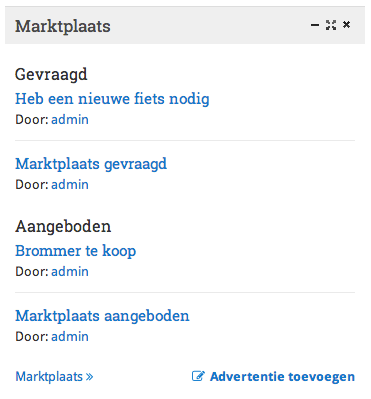
\includegraphics[scale=0.5]{img/blokken/marktplaatslijst.png}
\end{center}

\paragraph{Marktplaats gevraagd blok}

Toont een lijst met 5 items. De volgende onderdelen zijn zichtbaar: titel (klikbaar), geplaatst door, intro. Onderaan het blok staat een link naar de overzichtspagina en een link om een advertentie toe te voegen.

\begin{center}
	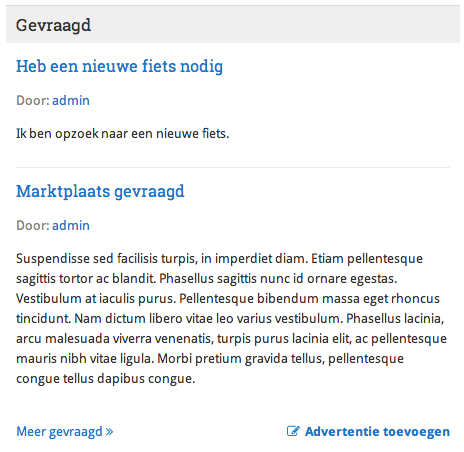
\includegraphics[scale=0.5]{img/blokken/marktplaatsgevraagd.png}
\end{center}

\paragraph{Marktplaats aangeboden blok}

Toont een lijst met 5 items. De volgende onderdelen zijn zichtbaar: titel (klikbaar), geplaatst door, intro. Onderaan het blok staat een link naar de overzichtspagina en een link om een advertentie toe te voegen.

\begin{center}
	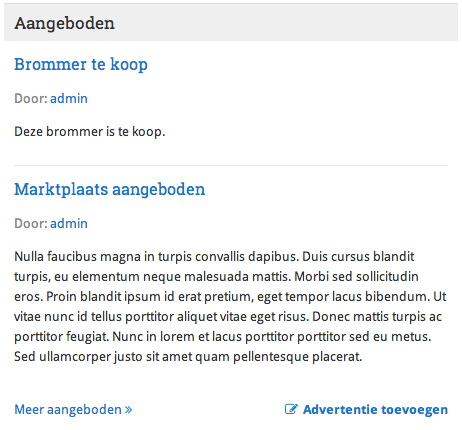
\includegraphics[scale=0.5]{img/blokken/marktplaatsaangeboden.png}
\end{center}

\paragraph{Marktplaats gevraagd pagina}

Toont een lijst met 10 items. De volgende onderdelen zijn zichtbaar: titel (klikbaar), geplaatst door, intro. Onderaan het blok staat de paginering en een link om een advertentie toe te voegen. Layout is te vergelijken met het \emph{Marktplaats gevraagd blok}

\paragraph{Marktplaats aangeboden pagina}

Toont een lijst met 10 items. De volgende onderdelen zijn zichtbaar: titel (klikbaar), geplaatst door, intro. Onderaan het blok staat de paginering en een link om een advertentie toe te voegen. Layout is te vergelijken met het \emph{Marktplaats aangeboden blok}

\paragraph{Nieuws teaserblok}

Toont een lijst met 10 nieuwsberichten. De volgende onderdelen zijn zichtbaar per nieuwsbericht: titel (klikbaar), thumbnail (klikbaar) en introtekst. Onderaan het blok zit paginering. Dit blok past optimaal in de middenkolom. Andere regio's zijn ook mogelijk het blok is responsive.

\begin{center}
	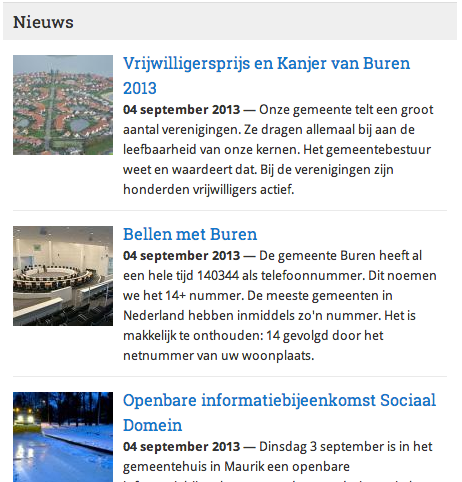
\includegraphics[scale=0.5]{img/blokken/nieuwsteaser.png}
\end{center}

\paragraph{Nieuws lijstblok}

Toont een lijst van 10 nieuwsberichten. De volgende onderdelen zijn zichtbaar per nieuwsbericht: titel (klikbaar), datum inzending en introtekst. Onderaan het blok zit staat een link naar de overzichtspagina en een link om nieuwsberichten toe te voegen wanneer de juiste rechten beschikbaar zijn. Dit blok past optimaal in de rechterkolom. Andere regio's zijn ook mogelijk het blok is responsive.

\begin{center}
	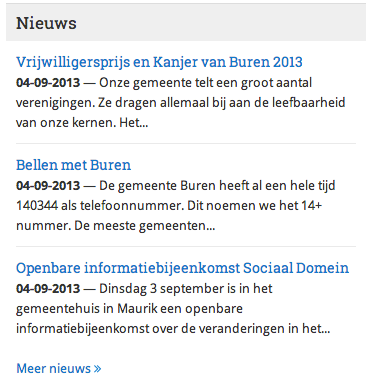
\includegraphics[scale=0.5]{img/blokken/nieuwslist.png}
\end{center}

\paragraph{Nieuws lijstblok + afbeelding}

Toont een lijst van 3 nieuwsberichten. De volgende onderdelen zijn zichtbaar per nieuwsbericht: thumbnail (klikbaar), titel (klikbaar) en datum inzending. Onderaan het blok zit staat een link naar de overzichtspagina en een link om nieuwsberichten toe te voegen wanneer de juiste rechten beschikbaar zijn. Dit blok wordt primair gebruikt op de voorpagina van het intranet.

\begin{center}
	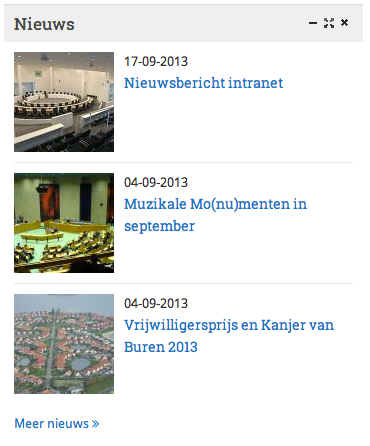
\includegraphics[scale=0.5]{img/blokken/nieuwsteaserimg.png}
\end{center}

\paragraph{Carrousel breed (9/12)}

Dit blok wordt gevuld door het content type slide die geplaatst worden in een nodequeue. Dit blok optimaal in de 9/12 verhoudingsregio.

\begin{center}
	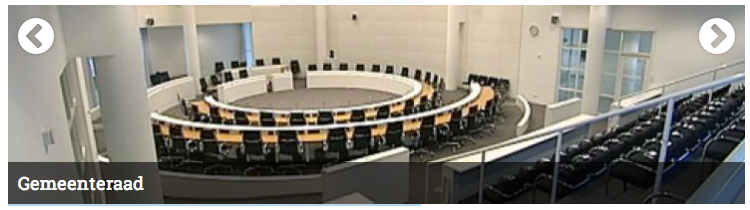
\includegraphics[scale=0.5]{img/blokken/carrouselbreed.png}
\end{center}

\paragraph{Carrousel smal (4/12)}

Dit blok wordt gevuld door het content type slide die geplaatst worden in een nodequeue. Dit blok optimaal in de 4/12 verhoudingsregio.

\begin{center}
	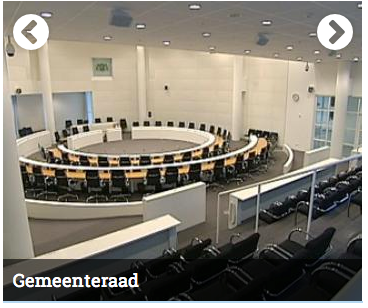
\includegraphics[scale=0.5]{img/blokken/carrouselsmal.png}
\end{center}

\paragraph{Personenblok intranet}

\paragraph{Personenblok internet}\label{personenblokinternet}

Toont een lijst met alle personen (content type) gegroepeerd per categorie.

\begin{center}
	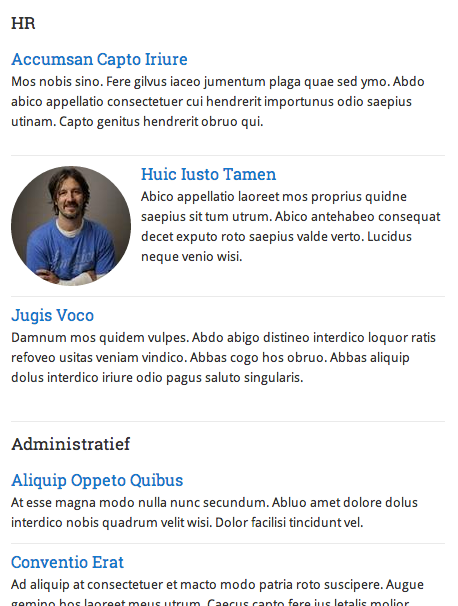
\includegraphics[scale=0.5]{img/blokken/personeninternet.png}
\end{center}

\paragraph{Teamledenblok}

Dit blok bestaat uit 3 kolommen gevuld met gebruikers die gekoppeld zijn aan de teamsite.

\begin{center}
	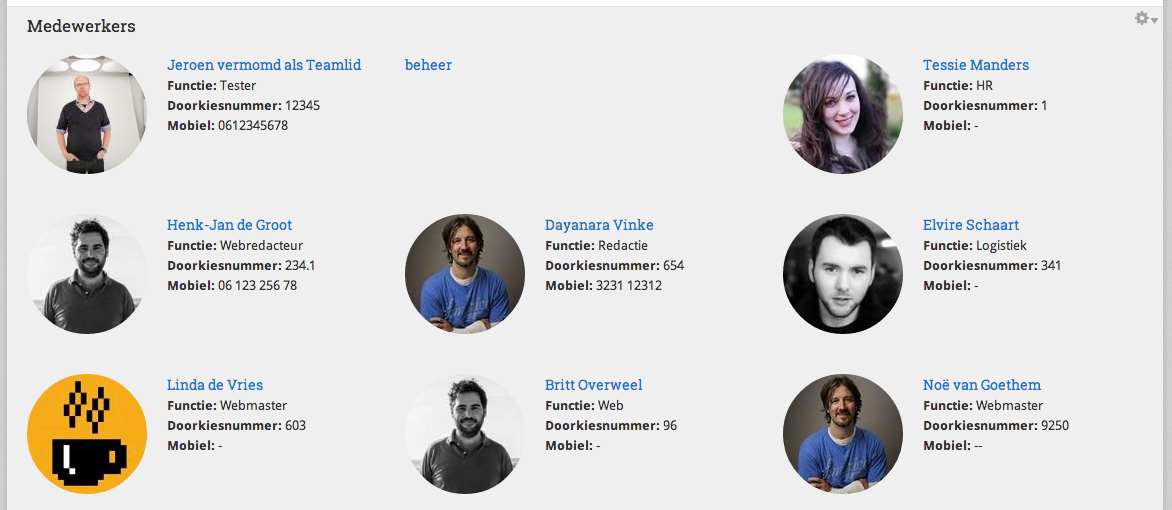
\includegraphics[width=\textwidth]{img/blokken/personenintranet.png}
\end{center}

\paragraph{Productenblok}

Dit is een blok dat wordt gebruikt om alle producten te tonen op alfabetische volgorde.

\begin{center}
	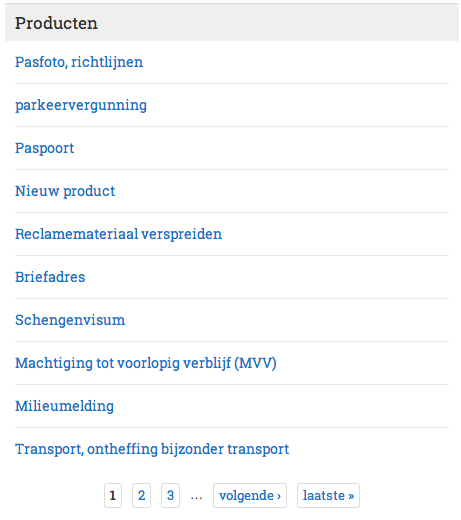
\includegraphics[scale=0.5]{img/blokken/producten.png}
\end{center}

\paragraph{Regelingenblok}

Dit is een blok dat wordt gebruikt om alle regelingen te tonen op alfabetische volgorde.

\begin{center}
	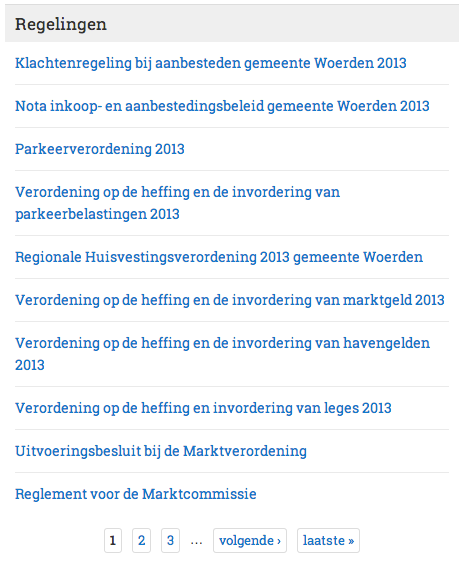
\includegraphics[scale=0.5]{img/blokken/regelingen.png}
\end{center}

\paragraph{Updatesblok}

Toont een lijst met 15 items van alle content dat geplaats/bijgewerkt wordt op het intranet en de teamsites. De volgende onderdelen zijn zichtbaar: Datum van plaatsen/bijwerken, titel (klikbaar), korte intro, tags.

\begin{center}
	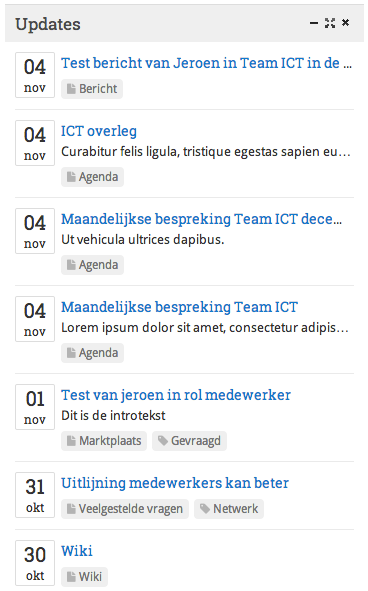
\includegraphics[scale=0.5]{img/blokken/updates.png}
\end{center}

\paragraph{Recent FAQs}

Toont een lijst met de 5 recente veelgestelde vragen. Deze lijst bestaat uit klikbare titels. Onderaan het blok staat een link naar de overzichtspagina en een link om een veelgestelde vraag toe te voegen mits de juiste rechten aanwezig zijn.

\begin{center}
	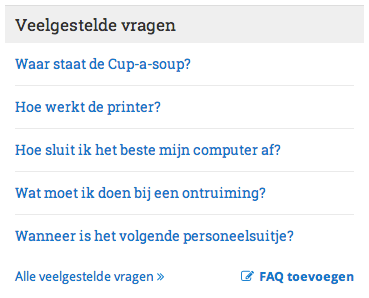
\includegraphics[scale=0.5]{img/blokken/faq.png}
\end{center}

\paragraph{Overige onderwerpenblok}

Toont 4 slides die gevuld zijn in een nodequeue.

\begin{center}
	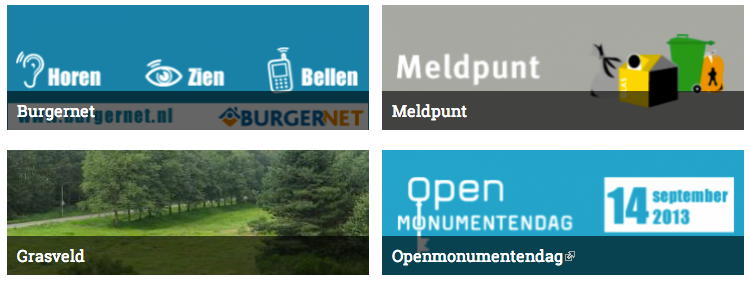
\includegraphics[scale=0.5]{img/blokken/onderwerpen.png}
\end{center}

\paragraph{Weblog blok}

Toont de laatste weblog. De volgende onderdelen zijn zichtbaar: titel (klikbaar), thumbnail, geplaatst door, intro. Onderaan het blok staat een link om een nieuw weblog toe te voegen mits de juiste rechten aanwezig zijn.

\begin{center}
	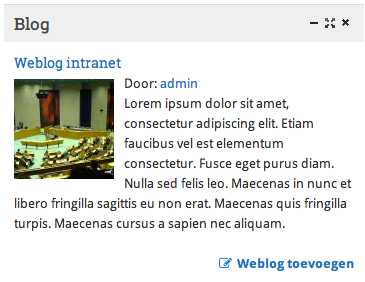
\includegraphics[scale=0.5]{img/blokken/blog.png}
\end{center}